\chapter{Vaadin}
Standardowe szkielety aplikacji do tworzenia stron WWW oferują tworzenie oprogramowania opartego o podejście żądanie-odpowiedź. Jest to model zupełnie inny, niż standardowy sposób pisania tzw. aplikacji desktopowych (czyli programowanie sterowane zdarzeniami), od których zaczynają swoją informatyczną kariere początkujący programiści . Niestety, zmiana modelu pisania programów wymaga przestawienia swojego myślenia. Na szczęscie istnieje jeszcze krok pośredni tzn. szkielety aplikacji, które umożliwiają tworzenie aplikacji internetowych poprzez programowanie sterowane zdarzeniami. Jednym z nich jest właśnie Vaadin - technologia zaproponowana przez promotora niniejszej pracy.

Vaadin jest szkieletem aplikacji, który umożliwia korzystanie z gotowych kontrolek i tworzyć aplikacje internetowe korzystające z AJAX jedynie za pomocą jednego języka programowania (może to być Java, ale także inne języki działające na wirtualnej maszynie Javy). Podejście Vaadina polega na tym, że każde zdarzenie wywołane po stronie klienta (przeglądarka WWW), jest przetwarzane po stronie serwera – co powoduje, że część aplikacji znajdująca się po stronie klienta nie zawiera żadnej logiki. Rozwiązanie wykorzystane w Vaadinie do odbierania żądań i wysyłania odpowiedzinie jest czymś nowym.

Elementem mającym styczność ze światem zewnętrznym jest serwlet (lub portlet) Vaadina, który tworzy obiekt usługi Vaadina. Do każdego połączenia usługa Vaadina przyporządkowuje sesje, w której obrębie przetrzymywane są zmienne. W ramach sesji użytkownik widzi wiele interfejsów (UI), które z kolei składają się z komponentów (omówione będą później), z którymi mogą być związani są nasłuchujący zdarzenia oraz model danych. 

\begin{figure} [H]
    \begin{center}
	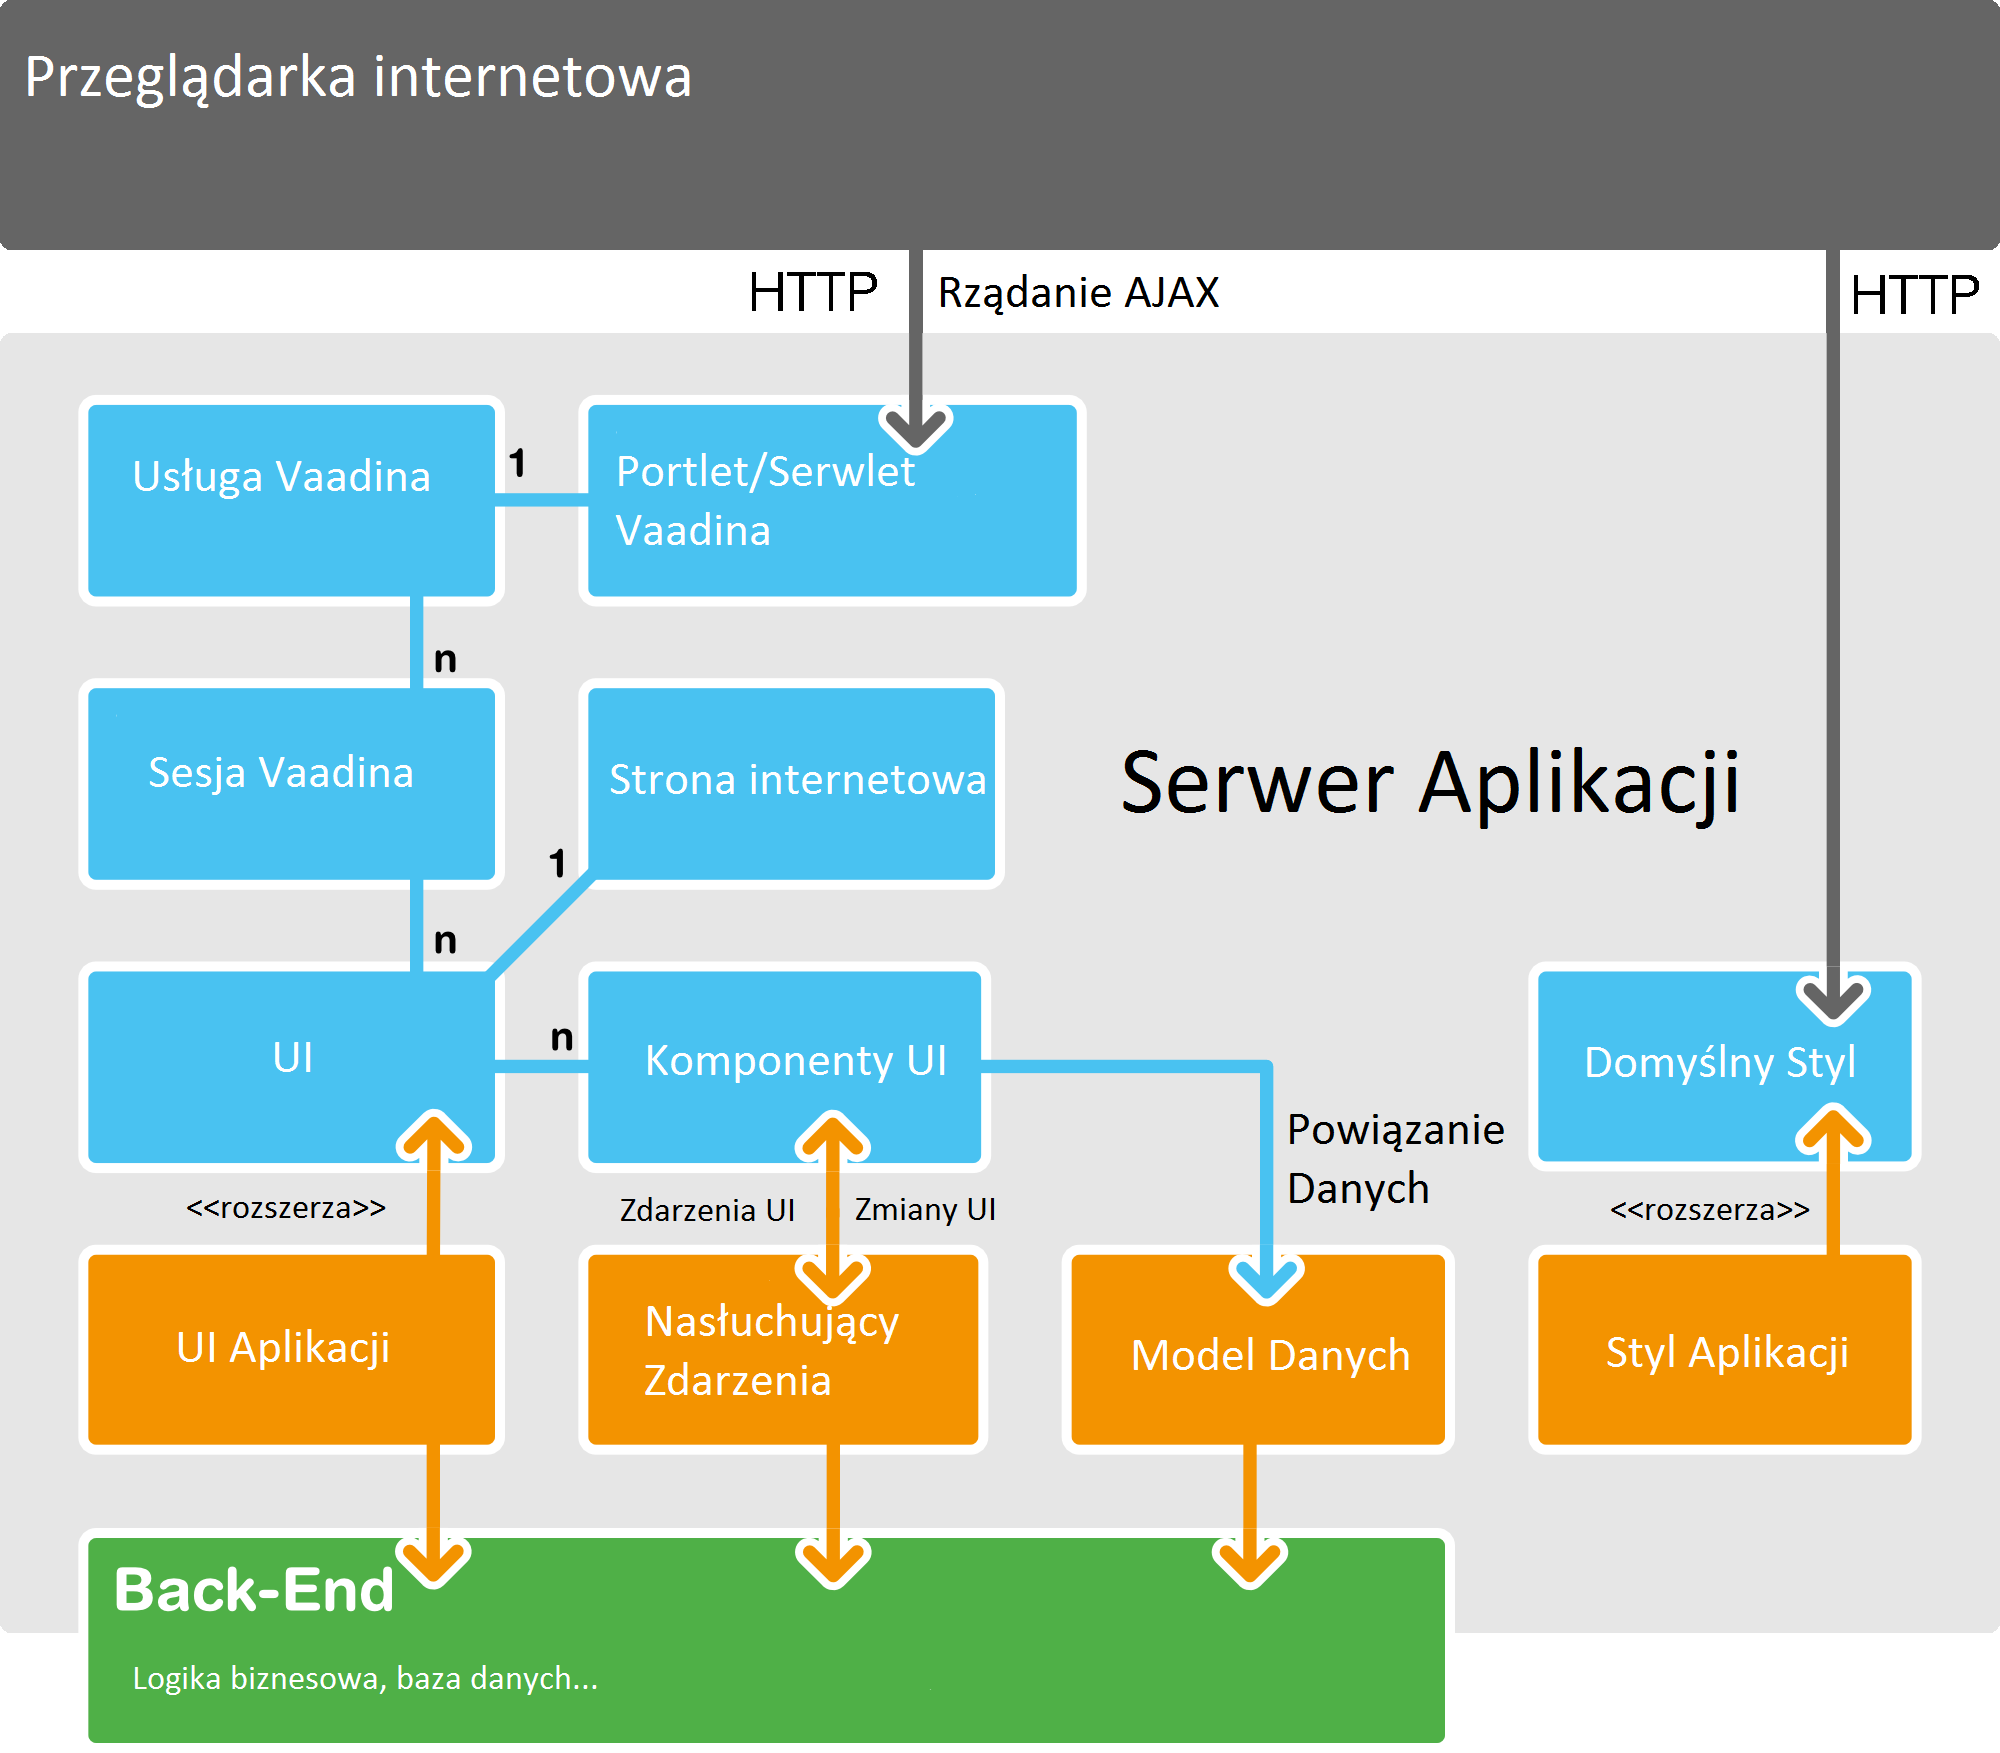
\includegraphics[scale=.3]{img/serverSide.png}
	\caption{Architektura szkieletu aplikacji Vaadin po stronie serwera}
	\label{serverVaadin}
    \end{center}
\end{figure}

\section{Zdalne wywoływanie procedury}
Cała tajemnica sukcesu Vaadin polega na zunifikowanym podejściu do obsługi zdarzeń. Każda kontrolka posiada swój łącznik, który jest podłączony do obiektu ApplicationConnection (jedna instancja na aplikacje) który odpowiada za komunikacje z serwerem po stronie klienta. Z drugiej strony natomiast występuje swego
rodzaju lustrzane odbicie – obiekt CommunicationManager jest połączony z każdym z komponentów. 

\begin{figure} [H]
    \begin{center}
	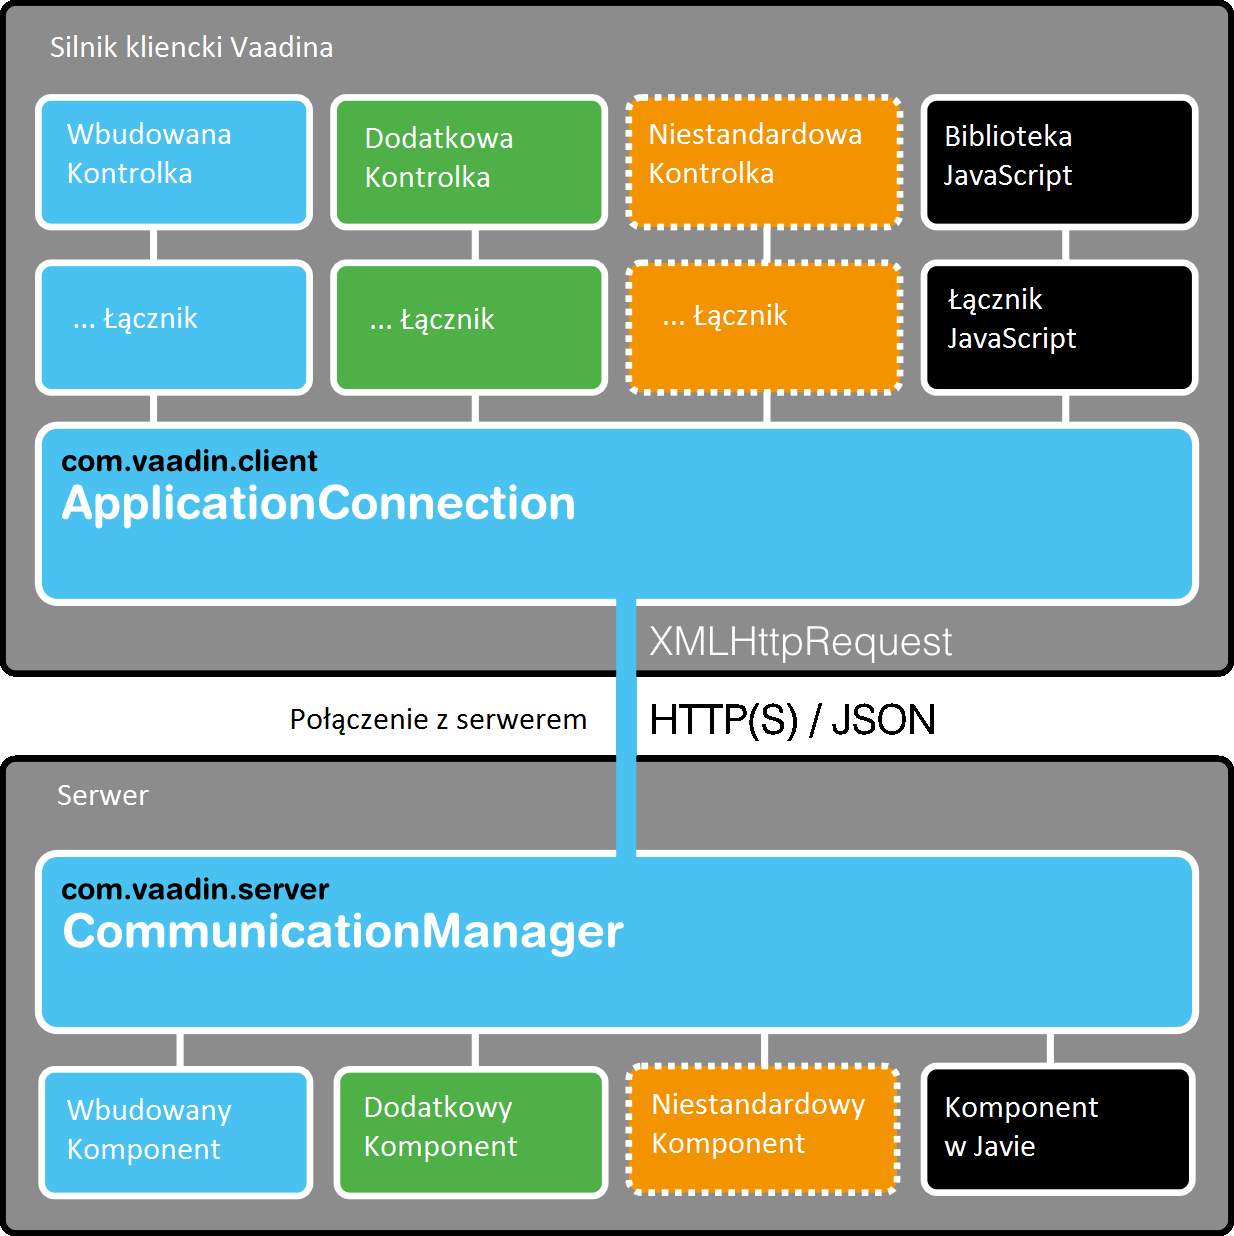
\includegraphics[scale=.3]{img/client.png}
	\caption{Komunikacja między kontrolką a komponentem}
	\label{architekturaVaadin}
    \end{center}
\end{figure}

Efekt ten można uznać za odmianę zdalnego wywoływania procedury – tzn. kontrolka wykonuje akcje związaną z nią przez JavaScript (jest to przezroczyste dla programisty) – komunikuje się przez WebService z serwletem Vaadina, który obsługuje żądanie, i w zależności od rezultatu – albo wysyła nową stronę do klienta albo asynchronicznie zmienia zawartość aktualnej.

\section{Architektura}
Do tej pory nie zostało to jeszcze powiedziane w sposób jednoznaczny – każdej kontrolce którą widzi użytkownik przyporządkowany jest po stronie serwera jeden komponent, który przechowuje stan kontrolki a także potrafi obsługiwać zdarzenia przez nią wygenerowane. 

\begin{figure} [H]
    \begin{center}
	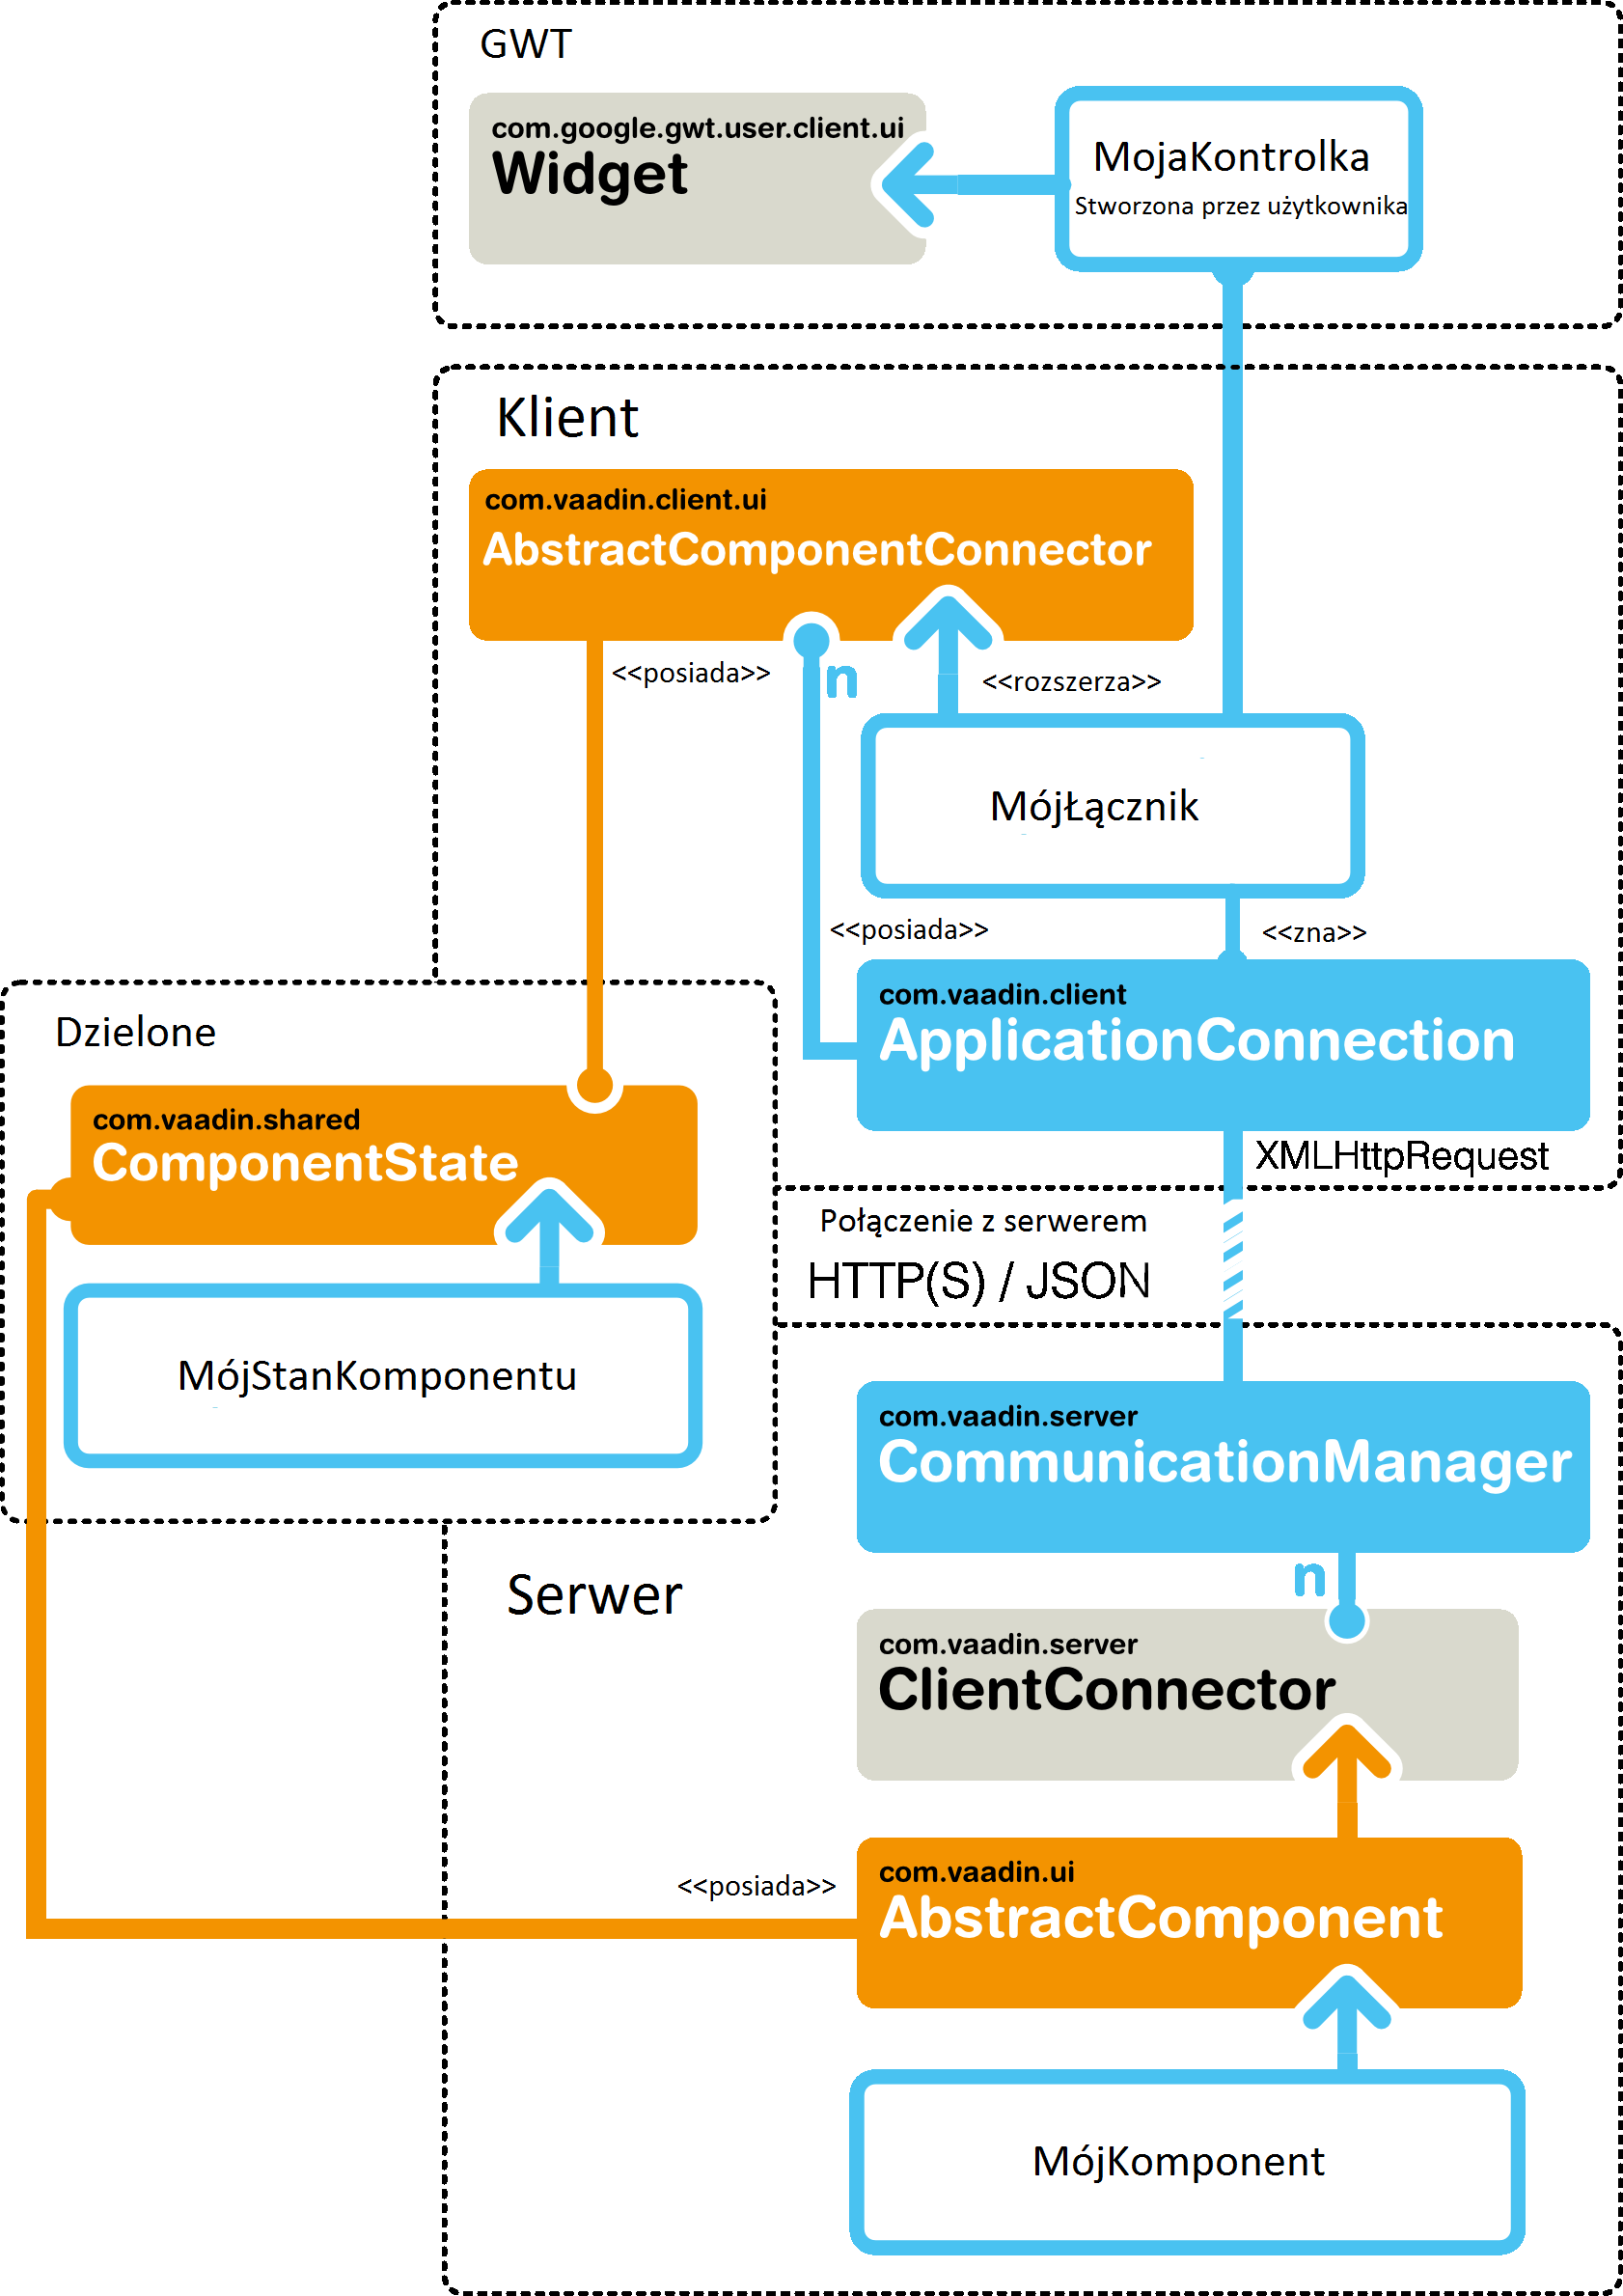
\includegraphics[scale=.2]{img/architektura.png}
	\caption{Implementacja połączenia kontrolki i komponentu}
	\label{clientVaadin}
    \end{center}
\end{figure}

Na powyższym schemacie przedstawiony jest sposób realizacji opisanego wcześniej podejścia. Z każdą kontrolką widzianą przez użytkownika związane są cztery klasy:
\begin{itemize}
\item Kontrolka – dziedzicząca po klasie Widget, definiująca co użytkownik widzi
\item Łącznik – który odpowiedzialny jest za przesyłanie informacji o zaistniałym zdarzeniu do serwera i synchronizacji stanu kontrolki
\item Komponent – klasa realizująca serwerową logikę kontrolki – realizuje reakcje na wygenerowanie zdarzenia, aktualizuje stan
\item Stan – klasa zawierająca informacje o aktualnym stanie kontrolki. 
\end{itemize}

Gdy zostanie wygenerowane zdarzenie przez kontrolkę po stronie klienta, łącznik przekazuje informacje o tym na stronę serwera do komponentu, który reaguje na tę zmianę. Możliwa jest zmiana stanu zarówno własnej kontrolki jak i innych kontrolek. Każdorazowa zmiana którejś z właściwości w obiekcie stanu powoduje asynchroniczną aktualizacje po stronie klienta.

\newpage
\section{Aplikacja po stronie klienta}
Jako jedną z zalet Vaadina zostało wymienione, że całość logiki znajdowała się po stronie serwera. Twórcy szkieletu aplikacji Vaadin zdają sobie jednak sprawę z tego, że część aplikacji potrzebuje natychmiastowych odpowiedzi (czyli nie ma czasu na czasochłonną komunikacje z serwerem przy każdym np. wciśnięciu klawisza) dlatego część zdarzeń powinna być obsługiwana po stronie klienta. 

Bardzo pomocny w tym celu okazuje się fakt, że Vaadin został stworzony jako obudowa dla GWT (Google Web Toolkit). Okazuje się, że istnieje możliwość skorzystania z kontrolek Google Web Toolkit w ramach aplikacji (istnieje także grupa kontrolek Vaadina dedykowanych specjalnie do tego rodzaju problemu).

\section{Nowe kontrolki}
Wielką zaletą szkieletu aplikacji który wybrałem jest spora liczba kontrolek będących w standardowym zestawie. Jeżeli jednak okazałoby się, że zbiór ten nie zawiera takiej, która jest potrzebna do zrealizowania funkcjonalności, warto udać się pod adres https://vaadin.com/download, pod którym do tej pory zostało opublikowanych prawie 400 nowych. 

Oczywiście może się okazać, że i w tej liście nie znajduje się odpowiednia kontrolka – w tym przypadku nie pozostaje już nic innego jak stworzyć nową. W ramach szkieletu aplikacji można tworzyć 4 rodzaje nowych kontrolek:
\begin{itemize}
\item Kontrolka złożona – składającą się z kilku istniejących kontrolek
\item Kontrolka rozszerzająca istniejącą (Vaadin) – zmieniająca właściwości / zachowanie tej kontrolki – np. zmiana tła pola tekstowego na niebieski
\item Kontrolka rozszerzająca istniejącą (GWT) – zaimplementowanie własnej kontrolki na podstawie istniejącej kontrolki z GWT
\item Całkiem nowa kontrolka, oparta o JavaScript/HTML – zaimplementowanie nowej kontrolki od zera również jest możliwe (choć skomplikowane).
\end{itemize}

\newpage
\section{Style}
Ludzie którzy tworzyli strony internetowe z wykorzystaniem HTML mogą być przyzwyczajeni do możliwości wyprowadzania elementów dotyczących wyglądu aplikacji poza zawartość kodu strony (CSS). Twórcy Vaadina prawdopodobnie dostrzegli dużą zaletę w tego typu podejściu, ponieważ w tym szkielecie aplikacji również jest to możliwe. Mechanizm ten jest wierną kopią kaskadowych arkuszy styli – można określać styl na każdym poziomie aplikacji, jednocześnie przykrywając go na poziomie niżej, np. kod powoduje że wszystkie tła w aplikacji będą koloru żółtego:
\begin{lstlisting}
.v-app {
	background: yellow;
}
\end{lstlisting}
Natomiast dopisując poniższy kod uzyskiwany jest efekt, polegający na tym że wszystko oprócz przycisków będzie posiadać żółte tło, które będą mieć tło kolorowane na niebiesko:
\begin{lstlisting}
.v-app .mybutton {
	background: blue;
}
\end{lstlisting}
\section{Powiązanie danych}
Główną rolą aplikacji internetowych jest przetwarzanie informacji. Ważnym elementem jest wyświetlanie danych wprowadzonych do bazy do tej pory, potrzebne jest także umożliwienie edycji / dopisania / usunięcia elementu. Tak samo jak każdy szanujący się szkielet aplikacji, Vaadin umożliwia uproszczenie tego procesu za pomocą powiązania danych (ang. Data Binding). W Vaadinie istnieją trzy wymiary, w których przechowywane są dane:
\begin{itemize}
\item Właściwość (ang. Property) – każda kontrolka posiada przypisaną do niej właściwość
\item Pozycja (ang. Item) – każdy formularz lub wiersz w tabeli posiada odpowiadającą mu pozycję
\item Pojemnik (ang. Container) – każdej tabeli odpowiada pojemnik przechowujący jej dane
\end{itemize}

Co daje powiązanie danych? Umożliwia to w prosty sposób edycje obiektów w bazie danych. Na przykład, wprowadzenie danych do formularza jest jednoznaczne z ustawieniem właściwości w obiekcie, dzięki czemu w wyniku np. kliknięcia przycisku dodaj, szkielet aplikacji dostarcza wypełniony już obiekt, gotowy do wprowadzenia do bazy danych. 
\newpage
Innym przykładem korzyści płynących z powiązania danych jest usunięcie wiersza z tabeli. Dzięki temu mechanizmowi minimalozowana jest praca polegająca na oprogramowywaniu przycisku usuń.


Ważnym elementem, w kontekście powiązania danych jest proces walidacji danych (szczególnie w formularzu). Vaadin umożliwia (jak większość szkieletów aplikacji) sprawdzenie poprawności wprowadzonych informacji, i w razie potrzeby wyświetla potrzebną informacje zwrotną o błędzie użytkownikowi. Walidacja odbywa się zgodnie ze standardem Java Bean Validation (JSR-303).

% ex: set tabstop=4 shiftwidth=4 softtabstop=4 noexpandtab fileformat=unix filetype=tex spelllang=pl,en spell: